<<<<<<< HEAD
\documentclass[10pt,a4paper]{article}
\usepackage[utf8]{inputenc}
\usepackage[german]{babel}
\usepackage[T1]{fontenc}
\usepackage{makeidx}
\usepackage{graphicx}
\usepackage{float}
\usepackage[automark]{scrpage2}
\author{M. Vierjahn und P. Kolschmieder}
\pagestyle{scrheadings}
\clearscrheadfoot
\cfoot[]{\pagemark}
\title{Ausarbeitung des Versuches K 1 im Fortgeschrittenen-Praktikum}
\begin{document}
\maketitle
\part*{Quanten-Hall-Effekt}
Versuchsdurchführung am 4. Dezember 2014\\
\section{Einleitung}
Der Quanten Hall Effekt wurde erstmals im Jahre 1980 von Klaus von Klitzing entdeckt und hat seitdem große Bedeutung in der Physik erlangt. Die Untersuchung von zweidimensionalen Elektronengasen ist damit weit vorangeschritten und der quantisierte Hall-Widerstand ist ein sehr genaues Maß als Widerstandsnormal geworden.\\
Ziel dieses Versuches war es, Ladungsträgerdichten und Beweglichkeiten in Abhänigkeit von drei unterschiedlichen Gatterspannungen jeweils in zwei verschiedenen 2DEG-Proben zu ermitteln. Des weiteren soll aus den Messungen die von-Klitzing-Konstante ermittelt werden und theoretische Erwartungen bei der Probe mit Antidot-Gitter beobachtet werden.\\ 
Im Versuch wurde eine GaAs-AlGaAs Heterostruktur verwendet mit n-dotiertem AlGaAs. Es wurden bei einer Probentemperatur von 4,2 K jeweils Quer- und Längs-Spannung über zunehmendem Magnet-Spulen-Strom geplottet (Magnetfeld: 0 - 5,6 Tesla). Es wurde ein Plot für die unstrukturierte Probe und einer für die strukturierte (mit Antidots) Probe zu jeweils drei Gatter-Spannungen erstellt. \\
Des weiteren wurden für die unstrukturierte Probe die Längswiderstände ohne Magnetfeld mit hoher Auflösung ermittelt und daraus die Beweglichkeit der Elektronen bestimmt. Um den Systematischen Fehler im Aufbau (Konstant-Spannung- statt Konstant-Strom-Quelle) zu ermitteln, wurden die Vorwiderstand-Spannungsabfälle tabellarisch bei verschiedenen Magnetfeldstärken festgehalten. \\
...Fazit... konnte alles beobachtet und innerhalb der Fehlergrenzen ermittelt werden...;-)
\section{Theoretische Grundlagen}
Für das Verständnis des Versuches sind sowohl Quantenmechanische als auch Grundlagen aus der Festkörperphysik notwendig. Im folgenden sollen die nötigsten Zusammenhänge dargestellt werden.
\subsection*{Klassische Betrachtung von Elektronen im E- und B-Feld}
Lässt man einen Strom I senkrecht zu einem Magnetfeld B durch einen Halbleiter fließen, so entsteht senkrecht zum Strom und Magnetfeld eine Querspannung $ U_H $, die Hall-Spannung genannt wird. Der Hall-Widerstand \begin{center}
$ R_H=\frac{U_H}{I}=\frac{B}{e*n_e}$
\end{center} 
steigt also im klassischen Falle linear mit dem Magnetfeld an (e: Elementarladung, $ n_e$: Ladungsträgerdichte) und aus der Steigung kann die Ladungsträgerdichte ermittelt werden.\\
Bei schwachem Magnetfeld ergibt sich ein Längswiderstand $ \rho _{xx}=\frac{U_{xx}}{I}*\frac{b}{l_{xx}} $, der von der Abmessung der Probe abhängt (b: Breite der Probe, $ l_{xx}$: Länge zwischen den Messstellen). Die Beweglichkeit der Elektronen ist als Verhältnis der Driftgeschwindigkeit $ v_d $ zum elektrischen Feld definiert und kann durch den Längswiderstand (ohne Magnetfeld), die Ladungsträgerdichte und die Elementarladung ausgedrückt werden:
\begin{center}
$\mu=|\frac{v_d}{E_{xx}}| =\left(\frac{1}{\rho _{xx}*e*n_e}\right) $.\\
\end{center} 
Bei einem starkem Magnetfeld werden die Elektronen in Zyklotron-Bahnen senkrecht zum B-Feld gezwungen, deren Radien vom Magnetfeld abhängen: 
\begin{center} 
$ R_{Zyclotron}=\frac{v_d}{\omega _c}=\frac{\hbar}{e*B}*\sqrt{2*\pi*n_e} $ 
\end{center} 
Dabei ist $\omega_c $ die Zyklotronfrequenz $ \omega _c=\frac{e*B}{m^*} $ wobei $ m^* $ die effektive Elektronenmasse ist.

\subsection*{Zweidimensionales Elektronengas}
In einer geeigneten Halbleiter-Heterostruktur, wie der im Versuch benutzten, entsteht nahe der Grenzschicht ein zweidimensionales Elektronengas. Dazu kommt es, da auf Grund Unterschiedlicher chemischer Potentiale die Leitungs- und Valenz-Bandkanten an der Kontaktfläche verbogen werden und somit ein quantenmechanischer Potentialtopf mit diskreten Energiespektren entsteht, der die Elektronen in einer Bewegungsrichtung einschränkt.\\
Wird nun ein starkes Magnetfeld angelegt, kommt es zu einer weiteren Quantisierung. Die Drehimpulsquantisierung bewirkt, dass nur bestimmte Zyklotronradien erlaubt sind. Das Lösen der Schrödingergleichung ergibt die zugehörigen Energieniveaus, die sogenannten Landau-Niveaus, 
\begin{center}
$E_n=\hbar\omega _c*(n+\frac{1}{2}) $
\end{center} 
welche über $ \omega _c=\frac{e*B}{m^*} $ vom Magnetfeld abhängen. Die Anzahl der besetzten Landau-Niveaus $ N_{L} $ ergibt sich aus der Tatsache, dass alle Elektronen auf die diskreten Niveaus aufgeteilt werden müssen zu
\begin{center} 
$ N_L=\frac{n_e*h}{2*e*B} $
\end{center}
und daraus der Füllfaktor $ \nu=\frac{n_e*h}{e*B} $, welcher die Aufhebung der Spin-Entartung berücksichtigt.\\
\subsection*{Quanten Hall Effekt und Shubnikov-de Haas-Oszillationen}
Bei genügend tiefen Temperaturen, so dass die thermische Streuung stark reduziert ist, verhält sich ein 2DEG anders als klassisch erwartet. Der Hallwiderstand nimmt ab einem ausreichenden Magnetfeld nicht mehr linear zu, sondern es bilden sich Plateaus in der Hall-Spannung bei denen $ R_H $ konstant bleibt. Diese werden mit zunehmendem Magnetfeld breiter und der Widerstandswert ist nur vom Füllfaktor $ \nu $ abhängig, der an den Plateaus ganzzahlig ist: 
\begin{center}
 $ R_H =\frac{R_K}{\nu}$,
 \end{center} 
 wobei
 \begin{center}
  $R_K=\frac{h}{e^2} $
\end{center} 
die von-Klitzing Konstante und h das Planksche Wirkungsqantum ist.\\ \\
Zugleich sind in der Längsspannung Oszillationen zu beobachten, bei denen der Längswiderstand zwischen Null und Maximalwerten oszilliert. Dieses Oszillationen werden  Shubnikov-de Haas-Oszillationen genannt. Die Minima liegen bei den Magnetfeldstärken, bei denen auch Plateaus in der Querspannung auftreten, die Maxima bei steil ansteigendem Hall-Widerstand.\\
Diese Phänomene lassen sich mit dem Modell der Randkanäle erklären, wobei angenommen wird, das der Strom im Falle des verschwindenden Längswiderstandes nur am Rand der Probe transportiert wird und dabei so gut wie keine Streuung der Ladungsträger auftritt da im inneren der Probe alle Elektronen stark lokalisiert sind. Bei steigendem Magnetfeld werden sukzessive Landau-Niveaus entvölkert was die starke Lokalisierung im Inneren der Probe aufhebt und damit die gesamte Probe zum Ladungstransport beiträgt. Durch die dadurch erhöhte Streuung von Ladungsträgern untereinander erhöht sich sowohl der Längs- als auch der Quer-widerstand. 
\section{Durchführung}
Der Probenhalter wurde bereits vor der Vorbesprechung teilweise in den He-Behälter eingeführt um unnötigen He-Verbrauch durch zu schnelles abkühlen zu vermeiden. Es wird die Probe D2 benutzt, welche im strukturierten Bereich runde Löcher als Antidots mit einer Gitterkonstante von 750nm enthält. Das Top-Gate ist eine 200nm dicke Goldschicht und es können die Spannungen -0,18V, 0V und 0,5V angelegt werden. Anhand einer nicht im Probenhalter befindlichen Probe wurde vom Betreuer der Aufbau selbiger erläutert. Die Anschlüsse am Probenhalter-Kopf waren wie in Abbildung \ref{Probe} \cite{1} gekennzeichnet. \\
\begin{figure}[H]
\begin{minipage}[b]{5.5 cm}
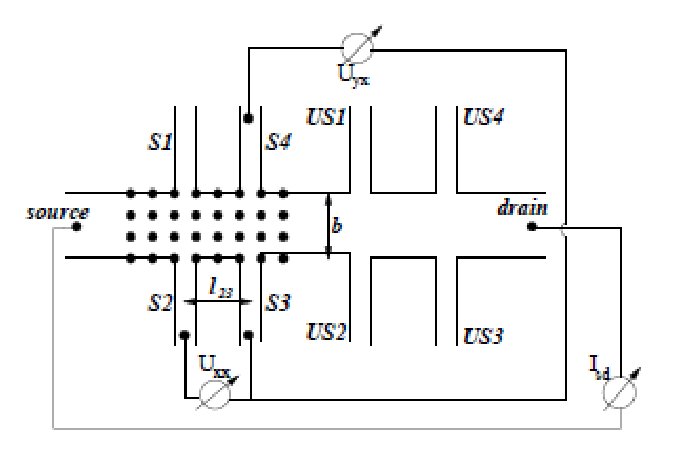
\includegraphics[scale=0.5]{Probenaufbau_cropped.pdf}
\caption{Probenaufbau}
\label{Probe}
\end{minipage}
\begin{minipage}[b]{5.5 cm}
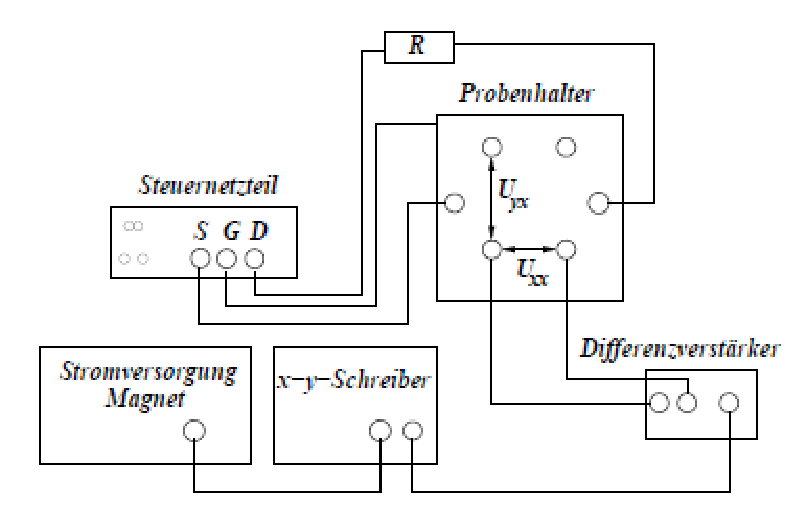
\includegraphics[scale=0.5]{Verkabelung_cropped.pdf}
\caption{Verkabelung}
\label{Verkabelung}
\end{minipage}
\end{figure}

 Die Verkabelung wurde gemäß Abbildung \ref{Verkabelung} \cite{1} durchgeführt und als die Probe mit Halter auf 4,2 K abgekühlt war (kein weiteres ausströmendes Helium aus dem Behälter), wurden die Geräte eingeschaltet und verschiedene Test-Plots gemacht um mit den Geräten vertraut zu werden und die optimalen Skalierungen für die verschiedenen Messungen am Plotter zu ermitteln.\\
Es ergaben sich hierbei einige physikalisch nicht sinnvolle Längsspannungsmessungen, bei denen Selbige deutlich unter die Nulllinie gerieten. Ein Umstecken der Kabel US2 $\leftrightarrow$ US3 und Umschalten am Plotter behoben das Problem bei der unstrukturierten Probe ohne echte Erklärung.
Auch bei der strukturierten Probe ergaben sich diese Probleme, ein Wechsel der Anschlüsse S2 $ \rightarrow $ S1 und S3 $ \rightarrow $ S4 mit veränderten offset am Plotter behob das Problem auch hierbei.
\subsection{Unstrukturierte Probe}
Es wurden als erstes die Längsspannungen an den Probenanschlüssen US2 und US3 gemessen. Zu jeder Gatter-Spannung wurde zunächst eine Null-Linie geplottet, indem der Signalverstärkereingang kurzgeschlossen wurde (und damit echte Null Volt vom Schreiber dargestellt wurden). Dann wurde das Magnetfeld linear von 0 bis 5,65 T erhöht und der Spannungsabfall $ U_{xx} $ dabei geplottet.\\
Diese Prozedur wurde für die Gatter-Spannungen  +0,5 V (rot),  0,0 V (grün) und -0,18 V (blau) durchgeführt, die Nulllinie der Gatter-Spannung 0 V und 0,5 V wurden übereinander gelegt. \\
Als nächstes wurden die Kabel am Probenhalter auf die Anschlüsse US1 und US2 gesteckt um die Querspannung $ U_{yx} $ zu plotten. Dies wurde wiederum für die drei Gatter-Spannungen durchgeführt, dabei wurde darauf geachtet, das die B-Feld-Achse mit der B-Feld-Achse aus der $ U_{xx} $ Messreihe übereinstimmt. Die Nullpunktlage in Y Richtung wurde frei gewählt, so das nicht übereinander geschrieben wird.\\
Die jeweiligen Skalierungs-Faktoren wurden auf dem Ausdruck festgehalten und die Achsen Beschriftet.\\ \\
Die Messung der Längsspannung bei B=0 wurde zudem noch für alle drei Gatter-Spannungen auf selbes Messblatt mit maximal möglicher Auflösung geplottet und entsprechend beschriftet.  
\subsection{Strukturierte Probe}
Die Messungen an der strukturierten Probe wurden auf die gleiche Weise wie bei der unstrukturierten Probe auf einem neuen Messblatt durchgeführt, die hoch aufgelöste Messung  von $ U_{xx} $ bei B=0 wurde hier nicht vorgenommen.
\subsection{Erfassung des Vorwiderstand-Spannungsabfall bei verschiedenen Magnetfeldern}
Es wurden tabellarisch zu jeder Gatter-Spannung der Spannungsabfall am Vorwiderstand bei den Magnet-Spulen-Strom 0A, 5A, 10A, 15A, 20A und 25A festgehalten.\\
\section{Auswertung}
	\subsection{ Fehlerbetrachtung}
	Zu Beginn der Auswertung werden die vorhandenen Fehlerquellen (systematische sowie statistische) des Versuches betrachtet.
\subsubsection{Systematische Fehler}
	 Für den als konstant angenommenen Strom I(B) durch die Probe existiert ein systematischer Fehler durch die Benutzung einer Konstant-Spannungsquelle. Dieser lässt sich aus den Messungen des Vorwiderstand-Spannungsabfalles bei verschiedenen B-Feldstärken ermitteln. Es gilt  
	 \begin{center} $ U_{Konst} = U_{R_V}(B) + U_{Probe}(B) = I(B) *(R_V + R_{Probe}(B))$
	 \end{center}
	 und mit 
	 \begin{center}
	  $ I(B) = \frac{U_{R_V}(B)}{R_V} $ 
	  \end{center} kann der Fehler $ \frac{\Delta I}{I(B=0)} = \frac{\Delta U}{U(B=0)} $ angegeben werden. Unsere Messung ergab ein maximales $\Delta U $ von 37 mV was einen maximalen systematischen Fehler des Stromes von 1,8 \% bei hohen Magnetfeldern ergibt. \\
	 Der Strom nimmt also mit steigendem B-Feld ab, eine klare Linearität wurde aber nicht erkannt und der systematische Fehler somit bei der Auswertung der Graphen nicht rechnerisch kompensiert. 
	\begin{table}[H]
 	\caption{Vorwiderstands-Spannungsabfall bei verschiedenen Spulen-Strömen}
\begin{center}	
	 \begin{tabular}{|c|c|c|c|c|c|c|}
	\hline 
    $U_{Gatter}$ [V] & 0 A & 5 A & 10 A & 15 A & 20 A & 25 A \\ 
	\hline \hline
	-0,18 & 1,999 & 1,994 & 1,985 & 1,977 & 1,962 & 1,970 \\ 
	\hline 
	0,00 & 2,001 & 1,998 & 1,993 & 1,987 & 1,985 & 1,963 \\ 
	\hline 
	0,50 & 2,000 & 1,997 & 1,990 & 1,986 & 1,980 & 1,972 \\ 
	\hline 
	\end{tabular}
\end {center}	
	\end{table}	
	\subsubsection{Statistische Fehler}
	Die Fehler der Mess-, Anzeige- und Ausgabegeräte wurden als klein angenommen.\\
	Aus den Angaben des Vorwiderstandes $ R_V = 1 M\Omega \ \ 5\% $ ergibt sich ein ebenso großer Fehler von 5\% für den Strom, für unsere Auswertung wurde der ebenfalls auf dem Vorwiderstand angegebene Wert von 993$ k\Omega $ benutzt, womit sich I=2,0 $ \pm 0,1 \mu A $ also $\frac{\Delta I}{I}=5\% $ ergibt. \\
	Eine Ablesegenauigkeit von $\pm$ 1 mm aus den Plots ergibt mit den jeweiligen Skalierungs-Faktoren absolute Fehler, die in den Auswertungs-Tabellen als solche angegeben werden. Dabei liegt die Ungenauigkeit in erster Linie in der Erfassung der genauen Lagen der Plateaus, Minima und Maxima. Erst bei Bedarf werden die absoluten Fehler in relative Fehler umgerechnet (Produkt von Fehlern entspricht der Summe der relativen Fehler, Addition von Fehlern entspricht der Summe der absoluten Fehler).\\
	Ebenso wurde bei den zu ermittelnden Steigungen und daraus resultierenden Berechnungen verfahren. \\
	Zum Beispiel berechnet sich der Fehler einer Messung der von-Klitzing-Konstante folgendermaßen:\\
	$(Ablesefehler: 0,1cm)*(Skalierung: 1\frac{mV}{cm})\rightarrow(Spannungsfehler: 0,1mV)\rightarrow(rel.Spannungsfehler: \frac{0,1}{13,6})\rightarrow(rel. Widerstandsfehler: \frac{0,1}{13,6}+\frac{\Delta I}{I})=\\(rel. Gesamtfehler)\rightarrow(Absoluter Gesammtfehler: 27,2*(rel.Gesamtfehler))\\ $

	\subsection{ Ladungsträgerdichte aus Steigung der Hallspannung} 
	Es wurden die klassischen Hall-Geraden auf die Graphen der Hall-Spannung gelegt, deren Steigungen abgelesen und tabellarisch festgehalten. Daraus wurde die Ladungsträgerdichte gemäß $ n_e = \frac{I}{e} * \left(\frac{dU}{dB}\right)^{-1}  $ berechnet: 

	\begin{table}[h]
 	\caption{Unstrukturierte Probe}
\begin{center}
	\begin{tabular}{|c|c|c|c|c|}
	\hline 
    $U_{Gatter}$ [V] & Steigung $\left[\frac{cm}{5T}\right]$ & range $\left[\frac{mV}{cm}\right]$ & $ \frac{dU}{dB} \left[ \frac{mV}{T} \right]$ & $n_{e} \left[\frac{10^{15}}{m^2}\right]$ \\ 
	\hline \hline
	-0,18 & 12,2$ \pm0,5 $ & 1 & 2,4$ \pm0,14 $ & 5,1$ \pm0,6 $ \\ 
	\hline 
	0,00 & 15,5$ \pm0,5 $ & 1 & 3,1$ \pm0,10 $ & 4,0$ \pm0,3 $ \\ 
	\hline 
	0,50 & 11,7$ \pm0,5 $ & 2 & 4,7$ \pm0,18 $ & 2,7$ \pm0,2 $ \\ 
	\hline 
	\end{tabular}
\end{center}
	\end {table}
	\begin{table}[h]
 	\caption{Strukturierte Probe}
\begin{center}
	\begin{tabular}{|c|c|c|c|c|}
	\hline 
    $U_{Gatter}$ [V] & Steigung $\left[\frac{cm}{5T}\right]$ & range $\left[\frac{mV}{cm}\right]$ & $ \frac{dU}{dB} \left[ \frac{mV}{T} \right]$ & $n_{e}$ $\left[\frac{10^{15}}{m^2}\right]$ \\ 
	\hline \hline
	-0,18 & . & 2 & . & . \\ 
	\hline 
	0,00 & . & 1 & . & . \\ 
	\hline 
	0,50 & . & 1 & . & . \\ 
	\hline 
	\end{tabular}
\end{center}
	\end{table} 
	 Die bei diesem Verfahren ermittelten Ladungsträgerdichten sind mit einer recht großen Ungenauigkeit behaftet. Eine genauere Kenntnis des Stromes würde dies deutlich verbessern, jedoch ergeben sich auch aus der Steigungs-Ablese-Ungenauigkeit Fehler von mehreren Prozent.\\
	 Der Systematische Stromfehler wirkt sich hier nur wenig aus, da die Steigung vor allem aus dem Plot bei schwachem Magnetfeld zeugt.\\
	\subsection{ Bestimmung der Plateau-werte  und zugehöriger Füllfaktoren}
	Aus den Plots der Hall-Spannung wurden die ab etwa 1,5 Tesla erkennbaren Plateau-werte ($ U_{xy} , B_{Plateau} $) abgelesen und gemäß $ R_\nu = \frac{U_\nu}{I} $ (und $ \nu = \frac{n_e * h}{e * B_{Plateau}} $  mit $ n_e $ aus 3.2) umgerechnet.\\ Die Füllfaktoren wurden schließlich derart gewählt, so das $ R_\nu = \frac{R_H}{\nu}$ mit $ R_H \approx $ konstant mit $\bf ganzzahligem \ \nu \rm $ gilt.:
	\begin{table}[H]
 	\caption{Plateau-Widerstände und Füllfaktoren der unstrukturierte Probe}
	\begin{tabular}{|c|r|c|r|r|c|c|}
	\hline 
    $U_{Gat.}$[V] & Plateau[cm]  & range$\left[\frac{mV}{cm}\right]$ & $ U_\nu $ [mV] & $ R_\nu [k\Omega] $ & $ \nu $ & $ R_H [k\Omega] $\\ 
	\hline \hline
	-0,18 & 13,6$ \pm0,1 $ & 1 & 13,6$ \pm0,1 $ & 6,8$ \pm0,4 $ & 4 & 27,2$ \pm2 $\\ 
	\hline 
	-0,18 & 6,9$ \pm0,1 $ & 1 & 6,9$ \pm0,1 $ & 3,45$ \pm0,3 $ & 8 & 27,6$ \pm2 $\\ 
	\hline 
	-0,18 & 4,6$ \pm0,1 $ & 1 & 4,6$ \pm0,1 $ & 2,3$ \pm0,2 $ & 12 & 27,6$ \pm3 $\\ 
	\hline 
	-0,18 & 3,4$ \pm0,1 $ & 1 & 3,4$ \pm0,1 $ & 1,7$ \pm0,2 $ & 16 & 27,2$ \pm3 $\\ 
	\hline \hline
	0,00 & 13,8$ \pm0,1 $ & 1 & 13,8$ \pm0,1 $ & 6,9$ \pm0,5 $ & 4 & 27,6$ \pm2 $\\ 
	\hline 
	0,00 & 9,3$ \pm0,1 $ & 1 & 9,3$ \pm0,1 $ & 4,65$ \pm0,3 $ & 6 & 27,9$ \pm2 $\\ 
	\hline 
	0,00 & 6,9$ \pm0,1 $ & 1 & 6,9$ \pm0,1 $ & 3,45$ \pm0,3 $ & 8 & 27,6$ \pm2 $\\ 
	\hline 
	0,00 & 5,5$ \pm0,1 $ & 1 & 5,5$ \pm0,1 $ & 2,75$ \pm0,2 $ & 10 & 27,5$ \pm2 $\\ 
	\hline \hline
	0,50 & 13,7$ \pm0,1 $ & 2 & 27,4$ \pm0,2 $ & 13,7$ \pm0,9 $ & 2 & 27,4$ \pm2 $\\ 
	\hline 
	0,50 & 9,2$ \pm0,1 $ & 2 & 18,4$ \pm0,2 $ & 9,2$ \pm0,7 $ & 3 & 27,6$ \pm2 $\\ 
	\hline 
	0,50 & 6,8$ \pm0,1 $ & 2 & 13,6$ \pm0,2 $ & 6,8$ \pm0,5 $ & 4 & 27,2$ \pm2 $\\ 
	\hline 
	0,50 & 5,5$ \pm0,1 $ & 2 & 11$ \pm0,2 $ & 5,5$ \pm0,5 $ & 5 & 27,5$ \pm2 $\\ 
	\hline 
	0,50 & 4,6$ \pm0,1 $ & 2 & 9,2$ \pm0,2 $ & 4,6$ \pm0,4 $ & 6 & 27,6$ \pm2 $\\ 
	\hline 
	\end{tabular}
	\end{table}
	In Unseren Messungen erhalten wir einen mittleres $ <R_H> $ von 27,5 $\pm2 k\Omega $, was den Literaturwert von 25,8 $ k\Omega $ deutlich überschreitet, welcher jedoch innerhalb unserer Fehlerabschätzung liegt. Auffällig ist, das $ R_H $ für alle Messungen zu hohe Werte annimmt.\\ 
	\subsection{Bestimmung der Ladungsträgerdichten aus den SdH-Oszillationen}
	Zur Bestimmung der Ladungsträgerdichten aus den Shubnikow de Haas Oszillationen wurden zunächst die Magnetfeldstärken zu den jeweiligen Minima und Maxima der gemessenen Längsspannung erfasst. Die Füllfaktoren aus 4.3 wurden den Minima zugeordnet, für die Maxima wurde entsprechend interpoliert.\\
	 Es wurden die Füllfaktoren über die reziproke Feldstärke aufgetragen und aus den so entstandenen Graphen die Steigungen $ (\frac{d\nu}{d\left(\frac{1}{B}\right)}) $ abgelesen.
	
	\begin{figure}[H]
  		\begin{minipage}[b]{5 cm}
  	 
   			 \includegraphics [scale=0.5]{Diagramm441_cropped.pdf} 
   			 \caption{Unstrukturiert} 
  		\end{minipage}
  		\begin{minipage}[b]{5 cm}
    		\includegraphics [scale=0.5]{Diagramm441_cropped.pdf}
    		\caption{Strukturiert}  
  		\end{minipage}
	 \end{figure}
	 
	  Mit $ n_e = \frac{e}{h} * (\frac{d\nu}{d\left(\frac{1}{B}\right)}) $ führt diese zu den Ladungsträgerdichten:
	\begin{table}[H]
	\caption{Ladungsträgerdichten aus SdH-Oszillationen}
\begin{center}
	 \begin{tabular}{|c|c|c|c|}
	\hline 
    $U_{Gat.}$ [V] & Steigung $\left[\frac{\nu}{\frac{1}{B}}\right]$ & $ \frac{\Delta\frac{1}{B}}{\frac{1}{B}} $ & $n_{e} \left[\frac{10^{15}}{m^2}\right]$ \\ 
	\hline \hline
	-0,18 & 23,5$ \pm0,5 $& 3\% & 5,7$ \pm0,3 $ \\ 
	\hline 
	0,00 & 19,3$ \pm0,5 $& 2\% & 4,7$ \pm0,2 $ \\ 
	\hline 
	0,50 & 12,0$ \pm0,5 $& 2\% & 2,9$ \pm0,2 $\\ 
	\hline 
	\end{tabular}
\end{center}
	\end{table}	 
	 
	\subsection{Bestimmung der Beweglichkeit der Elektronen aus der Längsspannung bei B=0}
	Zur Bestimmung der Beweglichkeit der Elektronen im 2DEG wurden die hoch aufgelösten Messung der Längsspannung ohne Magnetfeld ausgewertet und der Längswiderstand der Proben für jede Gatterspannung ermittelt $ \rho_{xx} = \frac{U_{xx}}{I} * \frac{b}{l_{xx}} $. Mit den Ladungsträgerdichten aus 4.4 wurde die Beweglichkeit gemäß $\mu = \frac{1}{(\rho_{xx} * n_e * n)}$ berechnet.
	\begin{table}[H]
	\caption{Beweglichkeit aus Längsspannungsabfall}
	\begin{tabular}{|c|r|c|r|r|r|r|}
	\hline 
    $U_{Gat.}$[V] & $U_{xx} [cm] $ & range$[\frac{\mu V}{cm}]$ & $U_{xx} [\mu V]$ & $\rho_{xx} [\Omega]$ & $ n_{e} \left[\frac{10^{15}}{m^2}\right]$ & $\mu [\frac{m^2}{Vs}]$ \\ 
	\hline \hline
	-0,18 & 15,0$ \pm0,1 $ & 2 & 30,0$ \pm0,2 $ & 20$ \pm1,1 $ & 5,7$ \pm0,3 $ & 55$ \pm 6 $ \\ 
	\hline 
	0,00 & 11,3$ \pm0,1 $ & 0,5 & 5,65$ \pm0,05 $ & 3,8$ \pm0,2 $ & 4,7$ \pm0,2 $ & 355$ \pm 38 $ \\ 
	\hline 
	0,50 & 9,2$ \pm0,1 $ & 0,2 & 1,84$ \pm0,02 $ & 1,2$ \pm0,1 $ & 2,9$ \pm0,2 $ & 1751$ \pm 200 $ \\ 
	\hline 
	\end{tabular}
	\end{table}
	\subsection{Vergleich der ermittelten Ladungsträgerdichten und Beweglichkeiten}
	Die aus den verschiedenen Messungen erhaltenen Ladungsträgerdichten sowie die ermittelten Beweglichkeiten wurden über der Gatter-Spannung aufgetragen:
	\begin{figure}[H]
	\centering
	\caption{Probenkennwerte in Abhängigkeit von der Gatter-Spannung}
	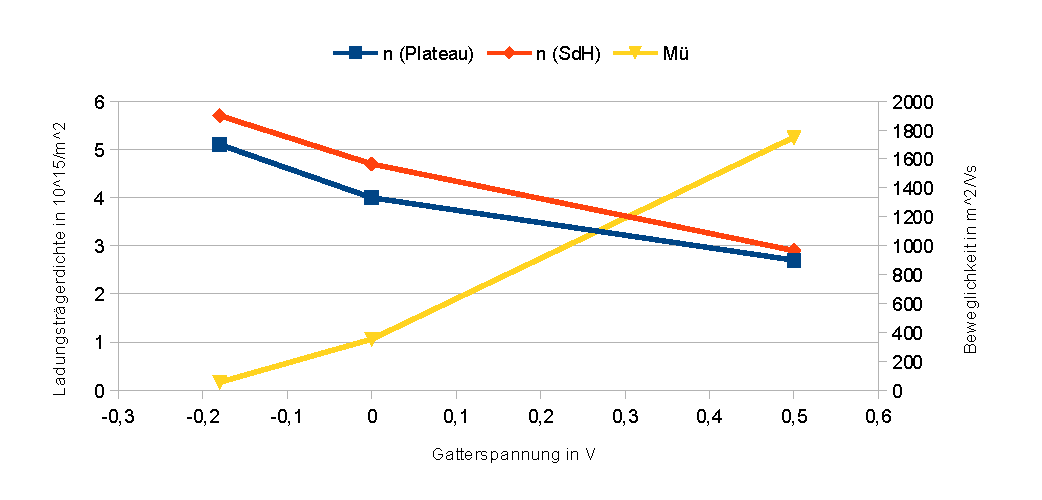
\includegraphics[scale=0.5]{diagramm46_cropped.pdf}
	\end{figure}
	
	Für die unstrukturierte Probe weichen die Ladungsträgerdichten aus den verschiedenen Messungen deutlich von einander ab, doch liegen diese Abweichungen innerhalb der Fehlergrenzen. Sie nehmen mit zunehmender Gatter-Spannung in etwa linear ab.\\
	Die Beweglichkeit verhält sich erwartungsgemäß umgekehrt, sie nimmt mit Steigender Gatter-Spannung zu. Durch eine geringere Ladungsträgerdichte im 2DEG erhöht sich die Stoßzeit $ \tau $ und somit auch der Leitwert $ \sigma _0= \frac{e^2*n_e*\tau}{m} $ . Das bedeutet eine Abnahme von $ \rho_{xx}(B=0)=(\sigma _0)^{-1} $ und damit eine verstärkte Zunahme der Beweglichkeit $ \mu = \frac{1}{n_e*e*\rho _{xx}} $.\\ \\
	Für die strukturierte Probe ...\\ \\
	
	Zwischen der Strukturierten und unstrukturierten Probe lassen sich folgende...\\ \\
	\subsection{von-Klitzing Konstante}
	Die von-Klitzing Konstante konnte in unserem Versuch zu 27,5 $\pm 2,0 k\Omega $ ermittelt werden, das ist eine magere Genauigkeit von 7\%. Um auf eine höhere Genauigkeit zu kommen, sollte der Vorwiderstand genau bekannt sein damit der Strom minimal Fehlerbehaftet ist. Eine Berücksichtigung des systematischen Fehlers in der Auswertung, oder besser eine Konstant-Stromquelle, würden die Genauigkeit weiter erhöhen.\\
Um den Literaturwert der Genauigkeit von 3,3 * $ 10^{-9} $ zu erreichen, müsste zudem die Erfassung der Hall-Spannung sehr, sehr genau und empfindlich sein.\\
\subsection{Genauere Betrachtung der Messung der strukturierten Probe}
Die Maxima in der Längsspannung zeugen von...
\\



\tableofcontents

\begin{thebibliography}{xxxxxxxxxxxxxxxxxxx}
   \bibitem[1]{1}Versuchsanleitung
\end{thebibliography}
\pagebreak

\begin {appendix}
\section*{Anhang}

\begin{figure}[hbtp]
\centering
	\caption{Plot der unstrukturierten Probe}
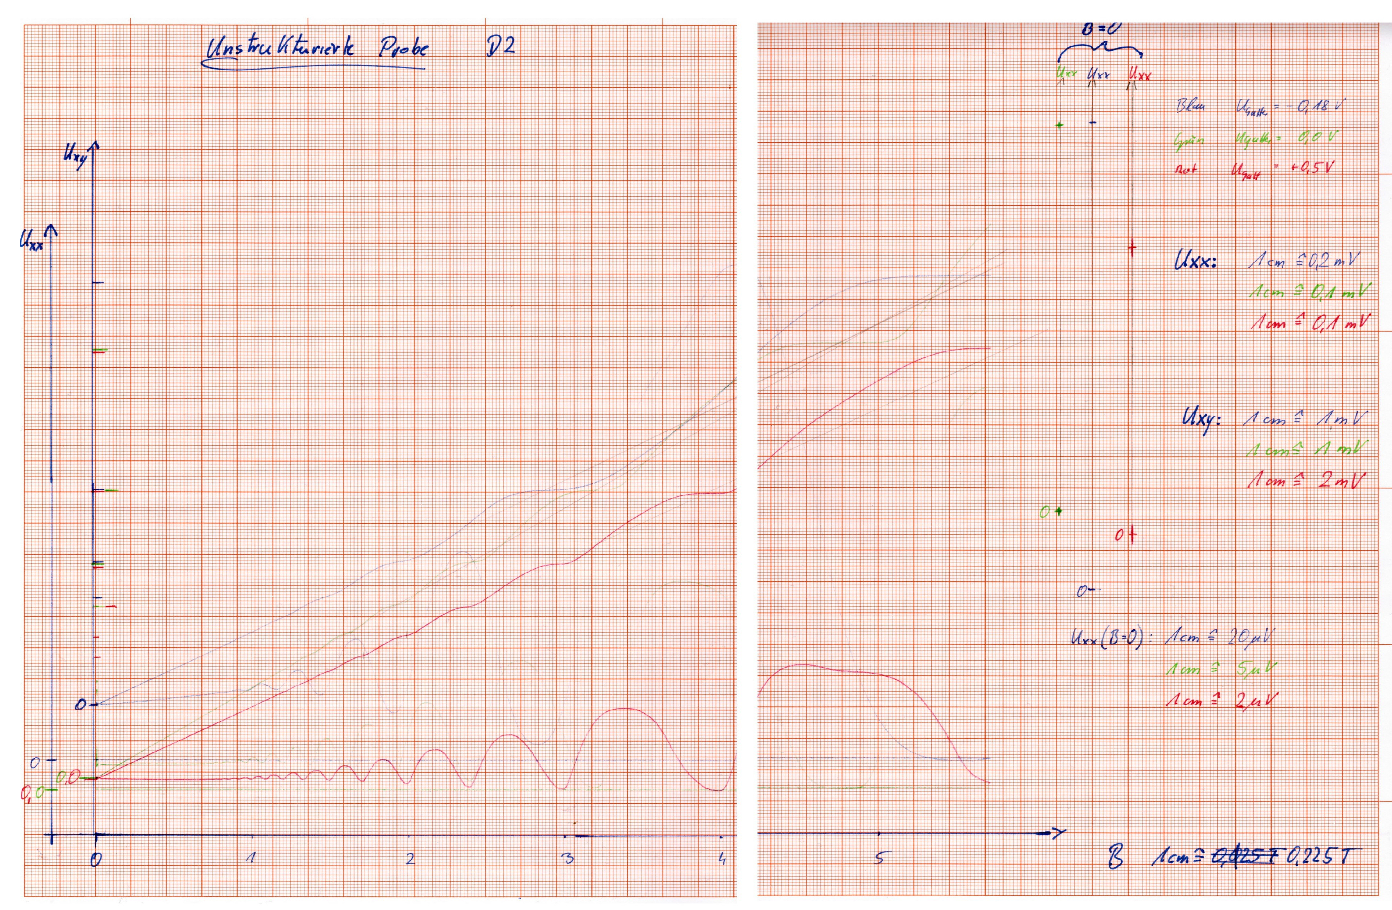
\includegraphics[scale=0.5]{plot_unstrukt_cropped.pdf}
\end{figure}

\end{appendix}

\end{document}

=======
QuantHallEff
============

versauswertung
>>>>>>> origin/master
